%%%%%%%%%%%%%%%%%%%%%%%%%%%%%%%%%%%%%%%%%%%%%%%%%%%%%%%%%%%%%%%%%%%%%%%%%%%%%
%%% LaTeX-Rahmen fuer das Erstellen von Masterarbeiten
%%%%%%%%%%%%%%%%%%%%%%%%%%%%%%%%%%%%%%%%%%%%%%%%%%%%%%%%%%%%%%%%%%%%%%%%%%%%%

%%%%%%%%%%%%%%%%%%%%%%%%%%%%%%%%%%%%%%%%%%%%%%%%%%%%%%%%%%%%%%%%%%%%%%%%%%%%%
%%% allgemeine Einstellungen
%%%%%%%%%%%%%%%%%%%%%%%%%%%%%%%%%%%%%%%%%%%%%%%%%%%%%%%%%%%%%%%%%%%%%%%%%%%%%

\documentclass[oneside,12pt,a4paper]{report}
%\usepackage{reportpage}
\usepackage{epsf}
\usepackage{graphics, graphicx}
\usepackage{latexsym}
\usepackage[margin=10pt,font=small,labelfont=bf]{caption}
\usepackage[utf8]{inputenc}
\usepackage[toc,page]{appendix}
\usepackage{amsmath, amssymb}
\usepackage{algorithm, algpseudocode}
\usepackage{siunitx}


\usepackage[round,comma]{natbib}\bibliographystyle{plainnat}
\usepackage[backref=section, hidelinks]{hyperref}
\usepackage{url}
\usepackage{makecell}

\usepackage{todonotes}

\newcommand{\figurewidth}{0.9\linewidth}
\newcommand{\done}[2][]{\todo[color=green!40, #1]{\textbf{Done:} #2}}


\textwidth 14cm
\textheight 22cm
\topmargin 0.0cm
\evensidemargin 1cm
\oddsidemargin 1cm
%\footskip 2cm
\parskip0.5explus0.1exminus0.1ex

% Kann von Student auch nach pers\"onlichem Geschmack ver\"andert werden.
\pagestyle{headings}

\sloppy

\begin{document}

%%%%%%%%%%%%%%%%%%%%%%%%%%%%%%%%%%%%%%%%%%%%%%%%%%%%%%%%%%%%%%%%%%%%%%%%%%%%
%%% hier steht die neue Titelseite 
%%%%%%%%%%%%%%%%%%%%%%%%%%%%%%%%%%%%%%%%%%%%%%%%%%%%%%%%%%%%%%%%%%%%%%%%%%%%
 
\begin{titlepage}
 \begin{center}
  {\LARGE Eberhard Karls Universit\"at T\"ubingen}\\
  {\large Mathematisch-Naturwissenschaftliche Fakult\"at \\
Wilhelm-Schickard-Institut f\"ur Informatik\\[4cm]}
  {\huge Master Thesis Computer Science\\[2cm]}
  {\Large\bf  Uncertainty-Aware Reinforcement Learning for Demand Response in Energy Systems\\[1.5cm]}
 {\large Ludwig Bald}\\[0.5cm]
  January 31, 2023\\[4cm]
{\small\bf Reviewers}\\[0.5cm]
  \parbox{7cm}{\begin{center}{\large Dr. Nicole Ludwig}\\
  {\footnotesize Wilhelm-Schickard-Institut für Informatik\\
	Universit\"at T\"ubingen}\end{center}}\hfill\parbox{7cm}{\begin{center}
  {\large Jun. Prof. Dr.-Ing.\\ Setareh Maghsudi}\\
  {\footnotesize Wilhelm-Schickard-Institut f\"ur Informatik\\
	Universit\"at T\"ubingen}\end{center}
 }
  \end{center}
\end{titlepage}

%%%%%%%%%%%%%%%%%%%%%%%%%%%%%%%%%%%%%%%%%%%%%%%%%%%%%%%%%%%%%%%%%%%%%%%%%%%%
%%% Titelr"uckseite: Bibliographische Angaben
%%%%%%%%%%%%%%%%%%%%%%%%%%%%%%%%%%%%%%%%%%%%%%%%%%%%%%%%%%%%%%%%%%%%%%%%%%%%

\thispagestyle{empty}
\vspace*{\fill}
\begin{minipage}{11.2cm}
\textbf{Bald, Ludwig:}\\
\emph{Uncertainty-Aware Reinforcement Learning for Demand Response in Energy Systems}\\ Master Thesis Computer Science\\
Eberhard Karls Universit\"at T\"ubingen\\
Thesis period: July 2022-January 2023
\end{minipage}
\newpage

%%%%%%%%%%%%%%%%%%%%%%%%%%%%%%%%%%%%%%%%%%%%%%%%%%%%%%%%%%%%%%%%%%%%%%%%%%%%

\pagenumbering{roman}
\setcounter{page}{1}

%%%%%%%%%%%%%%%%%%%%%%%%%%%%%%%%%%%%%%%%%%%%%%%%%%%%%%%%%%%%%%%%%%%%%%%%%%%%
%%% Seite I: Zusammenfassug, Danksagung
%%%%%%%%%%%%%%%%%%%%%%%%%%%%%%%%%%%%%%%%%%%%%%%%%%%%%%%%%%%%%%%%%%%%%%%%%%%%


\section*{Abstract}

Write here your abstract.
\newpage
\section*{Zusammenfassung}

Bei einer englischen Masterarbeit muss zus\"atzlich eine deutsche Zusammenfassung verfasst werden.


\newpage
\section*{Acknowledgements}

Write here your acknowledgements.

\cleardoublepage

%%%%%%%%%%%%%%%%%%%%%%%%%%%%%%%%%%%%%%%%%%%%%%%%%%%%%%%%%%%%%%%%%%%%%%%%%%%%%
%%% Table of Contents
%%%%%%%%%%%%%%%%%%%%%%%%%%%%%%%%%%%%%%%%%%%%%%%%%%%%%%%%%%%%%%%%%%%%%%%%%%%%%

\renewcommand{\baselinestretch}{1.3}
\small\normalsize

\tableofcontents

\renewcommand{\baselinestretch}{1}
\small\normalsize

\cleardoublepage

%%%%%%%%%%%%%%%%%%%%%%%%%%%%%%%%%%%%%%%%%%%%%%%%%%%%%%%%%%%%%%%%%%%%%%%%%%%%%
%%% List of Figures
%%%%%%%%%%%%%%%%%%%%%%%%%%%%%%%%%%%%%%%%%%%%%%%%%%%%%%%%%%%%%%%%%%%%%%%%%%%%%

% \renewcommand{\baselinestretch}{1.3}
% \small\normalsize

% \addcontentsline{toc}{chapter}{List of Figures}
% \listoffigures

% \renewcommand{\baselinestretch}{1}
% \small\normalsize

% \cleardoublepage

%%%%%%%%%%%%%%%%%%%%%%%%%%%%%%%%%%%%%%%%%%%%%%%%%%%%%%%%%%%%%%%%%%%%%%%%%%%%%
%%% List of tables
%%%%%%%%%%%%%%%%%%%%%%%%%%%%%%%%%%%%%%%%%%%%%%%%%%%%%%%%%%%%%%%%%%%%%%%%%%%%%

% \renewcommand{\baselinestretch}{1.3}
% \small\normalsize

% \addcontentsline{toc}{chapter}{List of Tables}
% \listoftables

% \renewcommand{\baselinestretch}{1}
% \small\normalsize

% \cleardoublepage

%%%%%%%%%%%%%%%%%%%%%%%%%%%%%%%%%%%%%%%%%%%%%%%%%%%%%%%%%%%%%%%%%%%%%%%%%%%%%
%%% List of abbreviations
%%%%%%%%%%%%%%%%%%%%%%%%%%%%%%%%%%%%%%%%%%%%%%%%%%%%%%%%%%%%%%%%%%%%%%%%%%%%%

% can be removed
% \addcontentsline{toc}{chapter}{List of Abbreviations}
% \chapter*{List of Abbreviations\markboth{LIST OF ABBREVIATIONS}{LIST OF ABBREVIATIONS}}

% \begin{tabbing}
% \textbf{FACTOTUM}\hspace{1cm}\=Schrott\kill
% \textbf{BLAST}\>Basic Local Alignment Search Tool \\
% \textbf{...} \> ...\\
% \end{tabbing}

% \cleardoublepage

%%%%%%%%%%%%%%%%%%%%%%%%%%%%%%%%%%%%%%%%%%%%%%%%%%%%%%%%%%%%%%%%%%%%%%%%%%%%%
%%% Der Haupttext, ab hier mit arabischer Numerierung
%%% Mit \input{dateiname} werden die Datei `dateiname' eingebunden
%%%%%%%%%%%%%%%%%%%%%%%%%%%%%%%%%%%%%%%%%%%%%%%%%%%%%%%%%%%%%%%%%%%%%%%%%%%%%

\pagenumbering{arabic}
\setcounter{page}{1}

%% Introduction
%%%%%%%%%%%%%%%%%%%%%%%%%%%%%%%%%%%%%%%%%%%%%%%%%%%%%%%%%%%%%%%%%%%%
% Einleitung
%%%%%%%%%%%%%%%%%%%%%%%%%%%%%%%%%%%%%%%%%%%%%%%%%%%%%%%%%%%%%%%%%%%%

\chapter{Introduction}\label{Introduction}
%- Because of climate change we switch the grid to renewable energies
Climate Change is the global challenge of our lifetime. Carbon introduced into the atmosphere when burning fossil fuels for human needs causes global warming, destabilizing the climate, ecosystems, and societies around the world.
In the Paris Agreement of 2015, governments have committed to an ambitious goal of drastically reducing carbon emissions to keep global warming from increasing beyond 2 °C, compared to 1990.
The latest report by the Intergovernmental Panel on Climate Change  urges governments to take stronger actions, or their previous commitment will not be reached \citep{portner2022ClimateChange2022}.
A key strategy for reducing carbon emissions from a range of sources is the combination of two measures: The first step is to electrify current processes that use fossil fuels, like replacing gas-fired furnaces with heat pumps. The second step is to replace carbon-intensive electricity generation with renewable options like solar and wind power.

%- renewable energies are less flexible than conventional energy supply
While much better for the natural environment, renewable sources of energy pose a challenge for a grid built for fossil fuels:
Unlike fossil-fuelled power plants, renewable power production depends on the weather, and it can not react flexibly to changes in demand.
As the share of installed renewable sources of electricity continues to grow, the reliability of the electricity supply will go down.

%- for a stable system, we need flexibility somewhere: supply, demand, or grid storage
In order to keep the grid stable, supply and demand must always be in balance. Before the green transition, this was achieved by flexible power generation: When demand was high, electricity producers were able to react and increase production.
This was incentivized by a complex and tightly regulated market constructed on top of the physical layer.
%    - supply doesn't work, so we need flexibility in demand and/or grid storage.
As the share of renewable power increases, fossil-fuelled plants remain the only market participants that can flexibly react to changes renewable production and demand for electricity.
When phasing out fossil-fuelled power generation, this flexibility needs to be provided by different parts of the system.

%    - in this thesis, I focus on demand-side flexibility.
There are dedicated electricity storage facilities that can react very quickly to stabilize the grid by storing and releasing energy as needed.
Grid-scale storage in Europe mainly consists of hydropower, which has been installed where mountainous geography allows, and capacity is limited \cite{gimeno-gutierrez2015AssessmentEuropeanPotential}.
More expensive battery-powered storage facilities are slowly being built, but are largely not cost-efficient in the current economic setting.
Therefore, there is a need for \emph{Demand Response}, or the ability of demand to flexibly respond to available electricity supply.

%- buildings are responsible for x\% of energy use
%- it makes sense for buildings to be able to react flexibly to changing conditions
Buildings use energy mainly for heating and cooling air and water supply.
Today, they are responsible for 17.5\% of global carbon emissions \cite{ritchie2020COGreenhouseGas}.
On the other hand, buildings often contribute to electricity production through photovoltaic panels. New buildings are often equipped with a battery, which enables them to more efficiently use their solar electricity.
Building electricity consumption is already largely automated and is therefore a prime candidate for automated demand response.

%- I use RL, an adaptive control algorithm, to provide this demand-side flexibility
%- cite RL in Demand Response
The \emph{Reinforcement Learning} (RL) family of control algorithms has shown promising performance in many control tasks, most notably video games (for example \cite{mnih2015HumanlevelControlDeep}), robotics \citep{latifi2020ModelFreeControlDynamicField} or wind power generation.% \citep{zhang2020ResearchAGCPerformance}.
RL is also being studied for controlling energy systems in buildings.
A popular simulation framework for this purpose is CityLearn \cite{vazquez-canteli2020CityLearnStandardizingResearch} introduce CityLearn, which proved a popular simulation framework for applying RL algorithms to building energy storage control.

\cite{wang2020ReinforcementLearningBuilding} find that the demand for data is a key challenge for applying RL for building control.
\cite{clements2020EstimatingRiskUncertainty} introduce \emph{Uncertainty-Aware Deep Q-Networks} (UA-DQN), a distributional RL algorithm based on DQN \citep{mnih2015HumanlevelControlDeep} that uses explicit uncertainty estimates for approximate Thompson sampling.
On a video game task, they show that this allows the algorithm to explore more efficiently, reducing the need for data.
In this thesis, I set out to test UA-DQN on a battery control task implemented with CityLearn.

%- my contribution is to apply uncertainty-aware RL, in the hopes of getting
%    - better performance 
%    - more robustness 
%    - risk-aware strategies
%- this contributes to our goal (flexibility in demand side).
The algorithm's better treatment of uncertainty should lead to overall better performance with less need for data, better robustness for novel data, and can even be leveraged for differently risk-aware charging and discharging strategies, all of which are important for building energy management.

This thesis is structured as follows: In chapter \ref{chap:background}, I motivate in more detail the need for Automated Demand Response. I introduce the theory of Reinforcement Learning and lay the foundations for the uncertainty-aware algorithm.
In chapter \ref{approach}, I present the uncertainty-aware algorithm, as well as a detailed description of the experimental setup.
I present the results in chapter \ref{results}.
A discussion and a short outlook conclude the thesis.

\cleardoublepage

%% 
%%%%%%%%%%%%%%%%%%%%%%%%%%%%%%%%%%%%%%%%%%%%%%%%%%%%%%%%%%%%%%%%%%%%
% Grundlagen
%%%%%%%%%%%%%%%%%%%%%%%%%%%%%%%%%%%%%%%%%%%%%%%%%%%%%%%%%%%%%%%%%%%%

\chapter{Background and related work}
  \todo[inline]{Give all the necessary background that is needed to justify and understand the problem and the approach.
  - comment on employed hardware and software
  - describe methods and techniques that build the basis of your work
  - review related work(!)
  - roughly 1/3 of thesis
  }

\section{The Electrical Grid and Flexibility}
% 1. Describe the goals and the structure of the Electrical Grid
The electrical grid is basic infrastructure that enables the function of our modern society.
It connects electricity consumers, from private consumers to heavy industry, with producers.
Historically, the entire system has been built for reliable large-scale power generation, overwhelmingly fuelled by coal and natural gas, together accounting for 67\% of Germany's electricity consumption in 1985, with 27\% provided by nuclear energy \cite{ritchie2022Energy}.

Climate change and the exit from nuclear power require a radical increase in the share of renewable electricity. As of 2021, renewable energy accounts for 40\% of electricity consumption in Germany \cite{ritchie2022Energy}.
An overview of the historical development is shown in figure \ref{fig:electricity_mix}

\begin{figure}
    \centering
    \frame{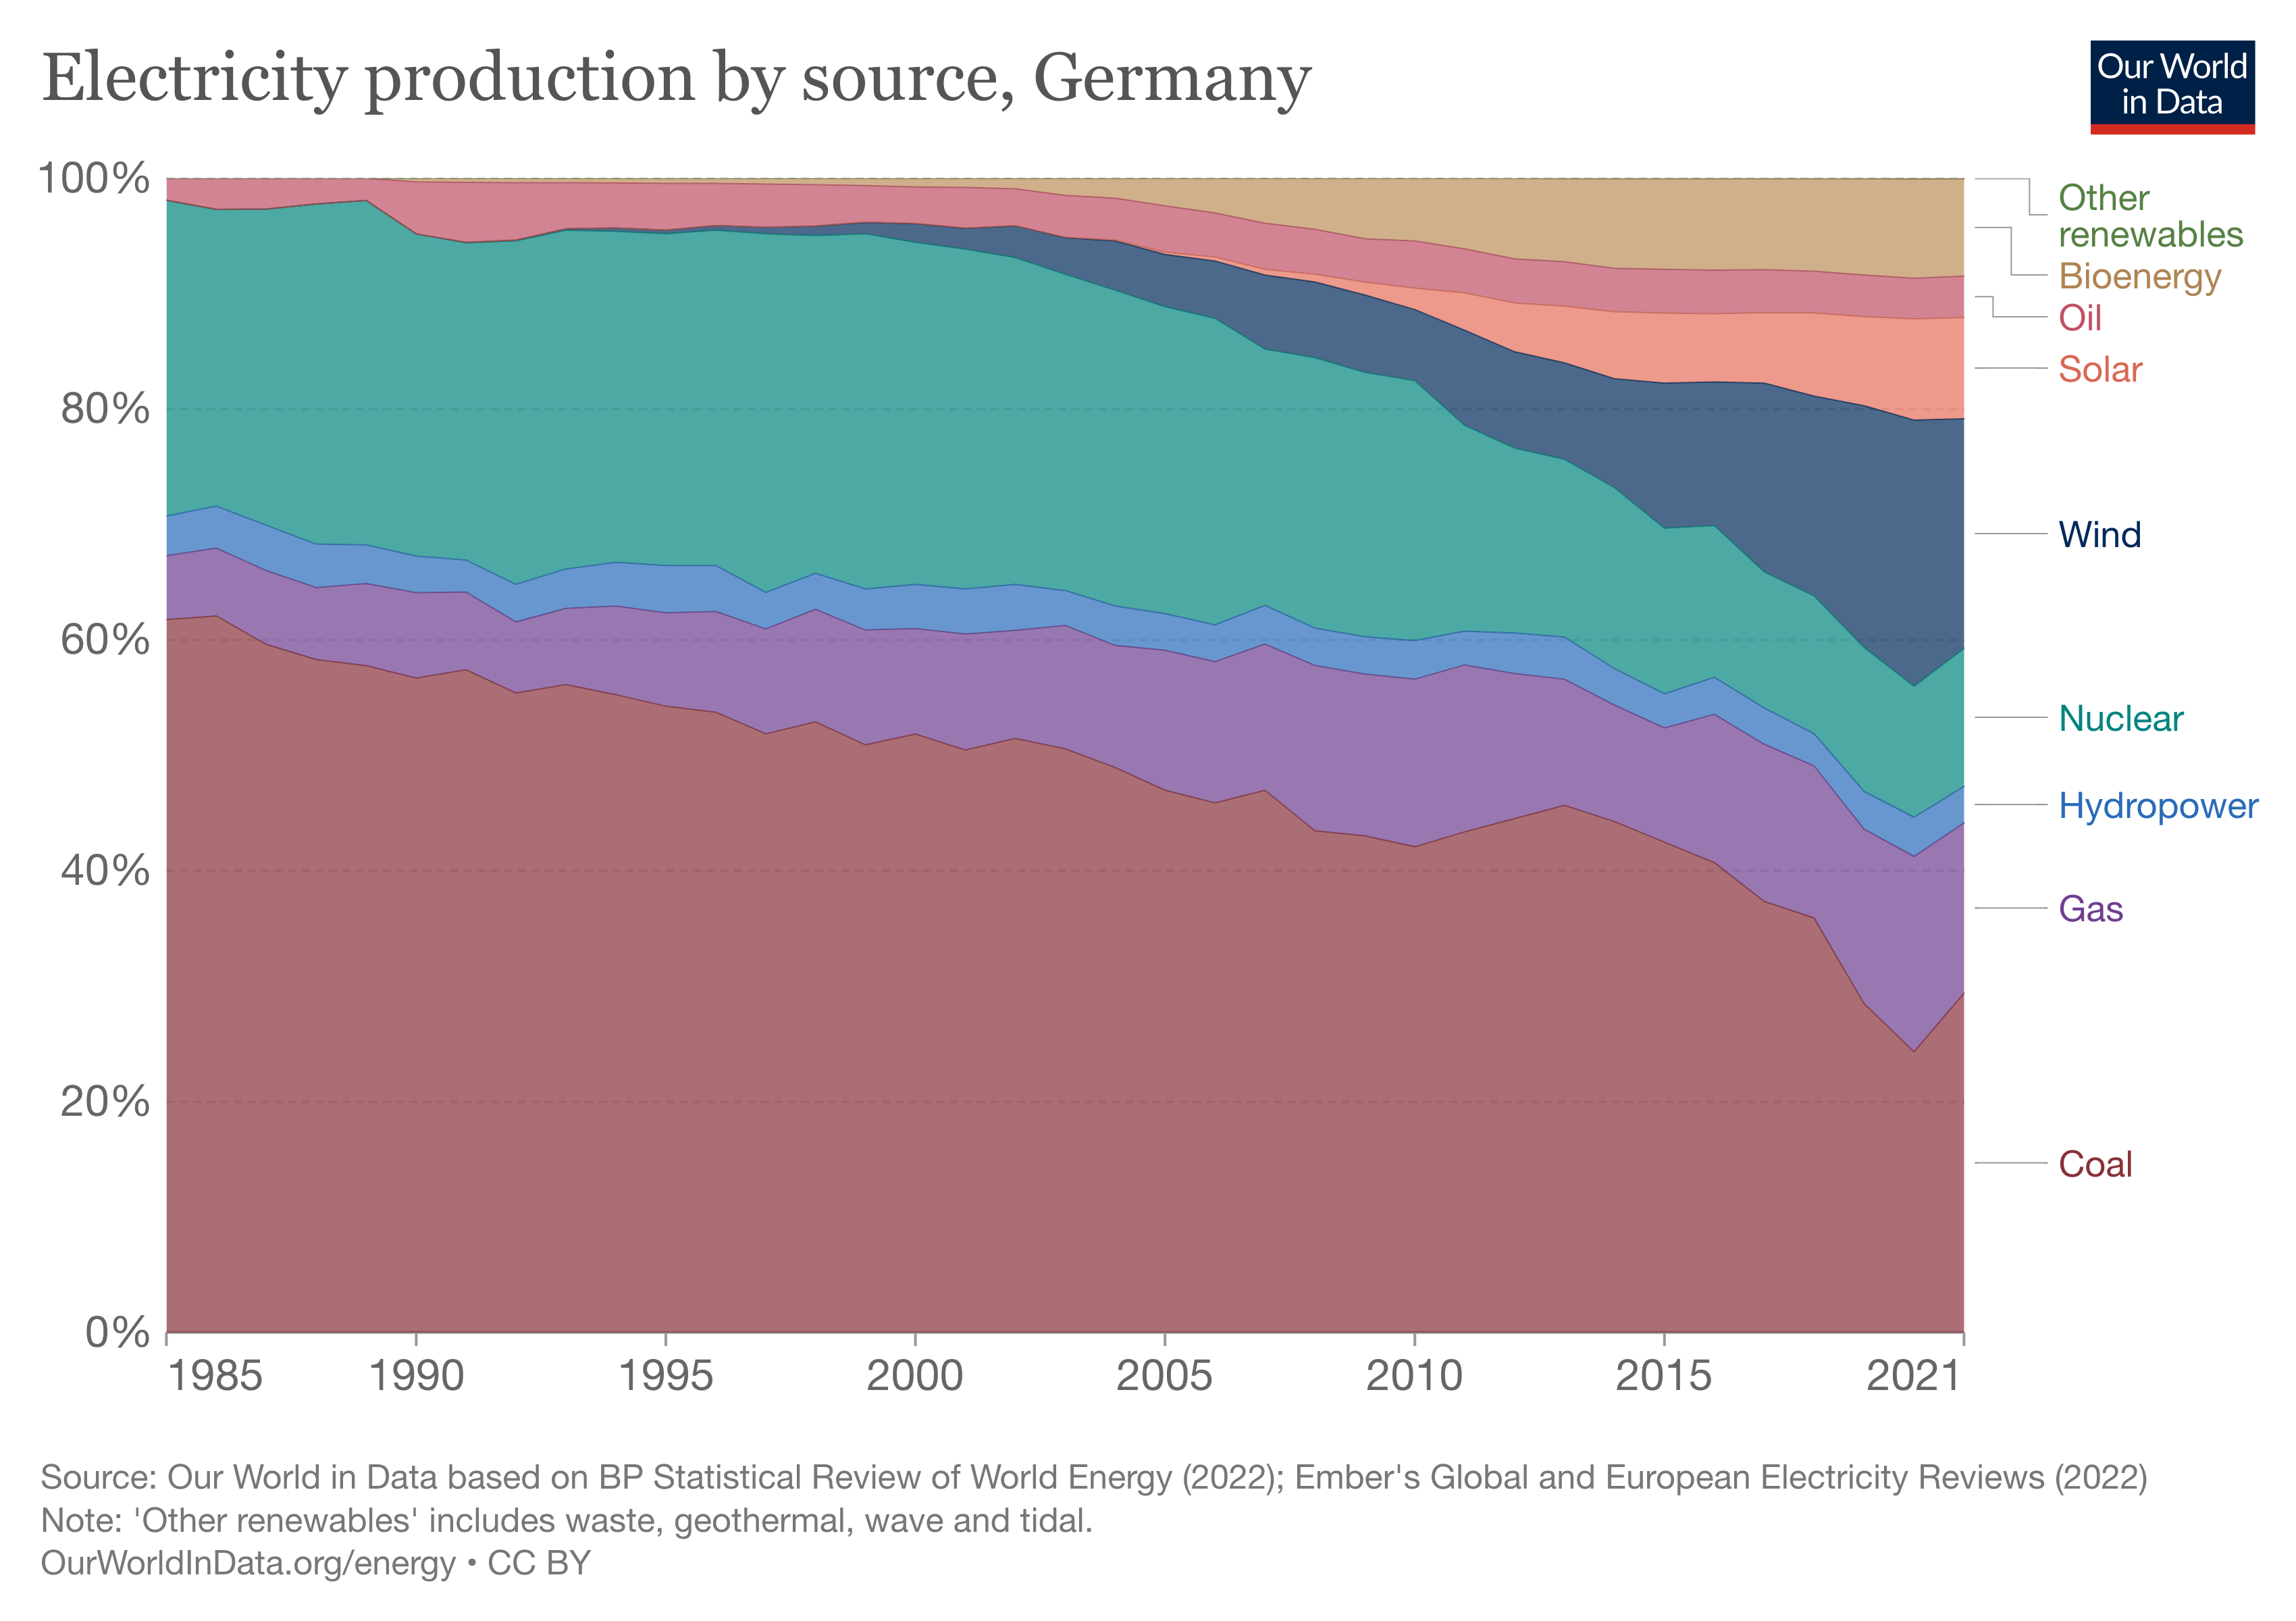
\includegraphics[width=\figurewidth]{figures/electricity_mix.png}}
    \caption{The share of renewable electricity has risen significantly from 1985 to 2021, while nuclear and fossil fuels have declined.}
    \label{fig:electricity_mix}
\end{figure}

While conventional energy generation can flexibly respond to demand, renewable energy depends on the weather.
It is therefore intermittent and harder to predict, see figure \ref{fig:flexibility}. To be able to meet demand, there is a new need for flexible backup power.
Natural gas plants are more environmentally friendly than coal plants and can be flexibly turned on and off in a matter of minutes.
As a result, the share of electricity powered by natural gas has risen along with renewables.

\begin{figure}
    \centering
    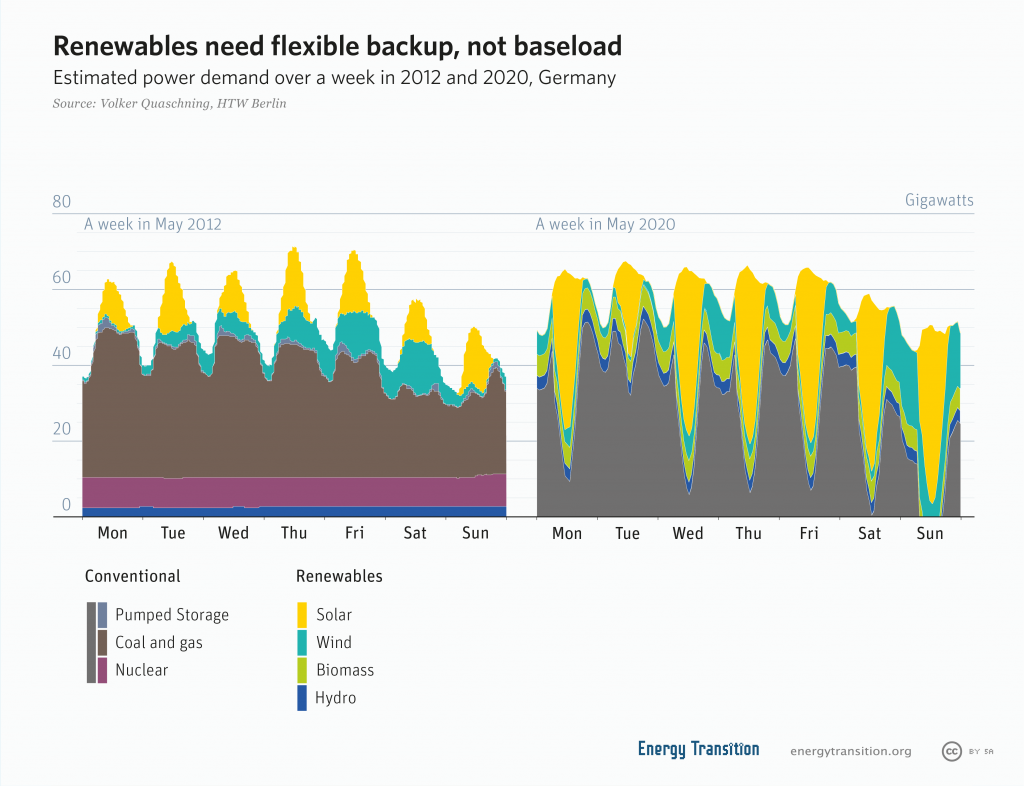
\includegraphics[width = \figurewidth]{figures/flexible_renewables.png}
    \caption{Renewable electricity is intermittent and hard to predict precisely. As the share of renewable electricity increases, the electrical grid needs to respond flexibly to meet demand.}
    \label{fig:flexibility}
\end{figure}


% 2. Describe Challenges posed by the energy transition
Another aspect of the energy transition is the electrification of many processes which previously used fossil fuels directly.
Internal combustion engine cars are being replaced by more efficient battery-powered electric cars and heating units that use natural gas or oil are being replaced by much more efficient electric heat pumps.
Many heat pumps can also be run in reverse to cool a building, which climate change makes more and more necessary, but this enables additional electricity demand in the summer.

The ongoing energy transition puts a lot of pressure on the grid.
On the one hand, the electricity supply is becoming less reactive, while on the other hand, many polluting processes are being electrified, causing additional demand.\todo{maybe give specific number}
During large future demand spikes, the total load on the grid could exceed current capacity. To cope, new transmission lines are being built, a costly and complicated process.

In order to both reduce reliance on fossil fuels and to keep the total load below grid capacity, there is a need for additional flexibility in the system.
A traditional source of flexibility has been pumped hydropower storage.
When there's unused electricity, it can be stored by pumping water uphill.
When needed, water can be released and used to generate electricity. 
Hydropower depends almost entirely on geography. There is almost no potential to develop more hydropower storage.

A different large-scale method of energy storage is batteries, which have only found limited use due to their cost. Hydrogen can also be used as a way to store and even transport energy, with several chemical processes currently being explored.
However, this method is also costly, and any produced hydrogen is probably worth more as a crucial chemical than as pure electricity storage.\todo{rephrase, cite}

As flexibility in electricity supply decreases, and centralized storage facilities remain too expensive, electricity demand needs to become more flexible.


\section{Demand Response}
% 3. Demand Side Flexibility
Both the inflexibility of renewable power generation and the limited capacity for centralized flexible energy storage leave one component of the electric system: In a renewable-dominated grid, demand needs to flexibly respond to changes in available supply.
In order to stabilize the grid, grid operators employ schemes to curb demand in case of exceptionally large pressure on the grid.
Large industrial consumers are paid in advance for shutting off their processes if needed.
As a matter of last resort, rolling blackouts are introduced to curb demand when electricity production can not keep up with consumption.
An electric grid designed for renewable energy needs more fine-grained coordination across a larger fraction of demand.

In order to implement demand response, electricity consumers need to be incentivized and able to adapt their processes to available supply.
Proposed incentive schemes for demand response include market-based solutions that feature a flexible electricity price and solutions of centralized control that pay out flat rewards for participation, as well as combinations of the two. \todo{cite}
In order to be able to react to changes in demand, electricity-consuming processes need to be aware of the current and future available supply.
This can be a human in the loop, deciding to shift a process to a time with cheaper electricity, or this can be automated.
For example, a private prosumer that produces solar electricity might prefer to run their washing machine only on sunny days when electricity is free to them.
However, this means the human needs to keep track of the weather and is put under additional cognitive load when planning this.

As stated before, the process of heating is being electrified.
While this increases the load on the electric grid, it is also a chance to provide flexibility:
When equipped with an intelligent and connected control system, the heating system can flexibly react to changes in price, using hot water tanks or the building itself as heat storage.
Similarly, when intelligently automated, the charging process of an electric car or a home battery can somewhat react to market conditions.
\todo{somehow mention coordination goals}

Technologically, this amounts to a control problem:
The controller's goals are to meet certain demands (like ensuring a comfortable living temperature) while minimizing cost. In the context of the larger system, there is the shared goal of coordination between different electricity-consuming processes.
This involves both an understanding of the dynamics of the controlled system and an understanding of how prices are likely to change.
Different technological approaches can be employed for this.
When system dynamics are known and prices change predictably, for example with fixed rates per time of day, an optimal rule-based controller can be derived. \todo{cite and make sure this is true!}
A rule-based controller has the advantage of being transparent and reliable, but it's not flexible enough to react to changing system and pricing dynamics.
Several adaptive control algorithms have been proposed for use in demand response. \todo{List some and cite}
\missingfigure{illustrate control problem}
\todo[inline]{
    notes on this section:
        - focus more on buildings
        - use the following review paper:
        - \cite{li2021EnergyFlexibilityResidential}, a review paper about energy flexibility in residential buildings
}


\section{Reinforcement Learning}

\todo[inline]{
    1. Explain RL Fundamentals
        1. Markov Decision Process
            1. Highlight stochasticity of transition and Reward functions
            2. Reward function?
            3. Mention generalizations: POMDP, (Multi-Agent MDP?), Non-stationary MDP
        2. Value Learning
            - Introduce the notion of a state value
            - Bellman updates
            - Q-Learning
            - Mention Policy Gradient methods
        3. Deep Q-Learning
            - introduce Fundamentals of Deep Learning? Deep RL is somewhat like using a POMDP?
            - Introduce further tricks employed by DQN
                - Replay Buffer
                - Dueling Q-Networks?
                - TD-Learning / Target Network
        4. Importance of Action Selection and Exploration strategies
            - Exploration vs. Exploitation Dilemma
            - Convergence guarantees
}


% 1. RL Fundamentals
\subsection{Reinforcement Learning Fundamentals}
Reinforcement Learning (RL) is a feedback-based learning paradigm derived from behavior learning in animals.
This section serves as a brief introduction to the topic.
Unless otherwise stated, this section is based on the textbook \cite{sutton2018ReinforcementLearningIntroduction}.
In Reinforcement Learning, there is a clear distinction between the learning agent and the environment.
The agent is able to observe the state of the environment and perform an action.
In turn, the environment is affected by the action and transitions into a new state according to its stochastic transition dynamics.
The environment passes the resulting state and a reward signal back to the agent.
Typically, the agent's goal is to select actions that obtain the maximum reward.
In an infinite environment, the objective is to maximize the expected value of the total discounted future reward.

The environment specifies the entire reinforcement learning task.
Formally, it is a discounted Markov Decision Process (MDP):
$$ \text{MDP} = (S, A, R, \gamma, p),$$
where $S$ is the set of possible states, $A$ is the set of possible actions, $R$ is the set of possible rewards, $\gamma$ is the discount rate and $p(s', r|s,a)$ is the probability distribution that specifies the environment dynamics.
It is important to note that an MDP has the Markov Property, i.e. the dynamics depend entirely on the state and action, there is no hidden state.
The state space can therefore also be called the observation space.

When modeling a real-world control problem, an MDP necessarily is a simplifying assumption.
In reality, state transitions often depend on outside influences or are non-stationary for other reasons.
In complex problems, the desired behavior is not obvious. Therefore, designing the reward function is often non-trivial.

\todo{Mention a few RL applications that can be used as examples}
\todo{Mention exploration/exploitation-dilemma here}

% 2. Towards DQN
\subsection{Q-Learning}
% - Value Learning
Some environment states are preferable to others.
Value Learning is a class of RL algorithms that builds on this intuition.
From a trajectory of state-action-observation-reward tuples that were generated while following a policy $\pi$, a Value Learning algorithm assigns each state the expected future discounted reward that will be received when the agent, in state $s$, continues to act according to $\pi$:

$$v_\pi(s) = \mathbb{E}[G_t | S_t=s] = \mathbb{E}[\sum_{k=0}^{\infty}\gamma^kR_{t+k+1} | S_t = s], \text{for all } s \in S$$

Similarly, one can define the value of taking an action in a certain state:
$$ q_\pi(s,a) = \mathbb{E}[G_t | S_t=s, A_t = a] = \mathbb{E}[\sum_{k=0}^{\infty}\gamma^kR_{t+k+1} | S_t = s, A_t = a]$$

This Action-Value Function or Q-function induces a greedy policy by evaluating $q(s,a)$ for the current state and all possible actions, and selecting the highest-expected reward action.
For the optimal policy $\pi_*$, the greedy policy induced by $q_{\pi_*}$ is $\pi_*$ itself.
For more detail on how the optimal policy can be approximated, please refer to \cite{sutton2018ReinforcementLearningIntroduction}.

%explain (e-greedy) action selection
%explain Q-Learning
A process that iteratively improves an initial Q-function is Q-Learning.
Its basic idea is that the Q-function can induce a better greedy policy than the one with which it was generated.
A Q-Learning step consists of taking an action $a$ in state $s$ according to the current greedy policy and performing a Bellman update on $q(s,a)$, using $\max_a{q(s',a)}$.
However, a slight modification needs to be made: To make sure all possible trajectories are explored, the $\epsilon$-greedy policy is used instead, which acts randomly with a small probability of $\epsilon$, and acts greedily otherwise.

\todo[inline]{
    Focus less on the idea of value learning.
    Instead, explain Tabular Q-Learning better
}

% - Deep Q-Learning
\subsection{Deep Q-Network}
\cite{mnih2015HumanlevelControlDeep} propose the Deep Q-Network algorithm (DQN), which is able to learn and play many video games better than humans.
DQN is a Q-Learning algorithm that acts according to an $\epsilon$-greedy policy.
It approximates the Q-function using a deep convolutional neural network, which is able to store complex information like video game dynamics.
The deep Q-network is optimized during every optimization step using stochastic gradient descent.

In order to arrive at a stable and efficient algorithm, DQN makes use of two notable modifications to standard online Q-Learning:
The first one, Experience Replay, stores past trajectories in a replay buffer.
During every optimization step, a minibatch of transitions $(s, a, r, s')$ is sampled from the replay buffer and used to compute the loss and gradient for the optimizer step.

The second modification is the use of a separate target Q-network.
The loss that is minimized is
$$ ((R_j + \gamma \max_a{\hat{q}(s',a)}) - q(s,a))^2$$
Instead of using the Q-network $q(s',a)$ as the target Q-value, DQN uses $\hat{q}(s',a)$.
$hat{q}$ is a lagging copy of the Q-network that is updated after several optimization steps.
This improves the stability of the algorithm.



% Uncertainty, Exploration vs Exploitation
\subsection{The Reward Distribution}
\todo[inline]{
    - Introduce the idea of Thompson sampling
        - requires a distribution instead of an expected Q-Value.
            - give formula for the q-distribution
    - Learn distributions: QR-DQN and \cite{azizzadenesheli2018EfficientExplorationBayesian}
    - 
    - If you do not have uncertainty, what can you do?
    - decay epsilon
    - use boltzmann sampling
    - Talk about how DQN treats uncertainty. (With epsilon-decay)

    - Introduce epistemic and aleatoric Uncertainty and their significance for action selection.
        - The uncertainty in the learned return distribution is caused both by inherent stochasticity of the environment and epistemic uncertainty.
        - Optimal action selection depends only on the epistemic uncertainty. If the goal remains to maximize the expected return overall, risk-averse things should happen too.
        - mathematically define them (variance of the Q estimator?)
        - \cite{hullermeier2021AleatoricEpistemicUncertainty} explain the concept.
        - 

}

Reinforcement Learning algorithms need to solve the Exploration/Exploitation-Dilemma.
When interacting with the environment, they need to balance between the value of gathering new information and the value of acting greedily according to their current knowledge.
The $\epsilon$-greedy policy exposes the parameter $\epsilon$ as a direct way to control this trade off.
Because the algorithm has the most to learn at the beginning, $\epsilon$ is commonly set to a high value in the beginning and then decayed over time.
Most Reinforcement Learning algorithms don't provide an explicit measure of uncertainty, which could be used to dynamically adapt this practice to the environment at hand.


\section{Reinforcement Learning for Building Demand Response}
\todo[inline]{
- Motivation: RL is a class of control algorithms that has been successfully applied to DR.
- Why is building DR a particularly good fit for RL?
- Mention prior work: When has RL been applied to building demand response?
    - paper 1: 
    - paper 2: 
    - paper 3: 

    - (Mention related work: applied algorithms and their results)
    - (Other Frameworks and available data, including CityLearn, real-life applications)
}

\subsection{CityLearn} % The basis for the environment.
\todo[inline]{
    1. Introduce and Explain CityLearn (cite)
        - What is it?
            - A simulation framework for constructing demand response environments for RL
        - What are its main contributions?
            - Provide an accessible entry point for RL researchers for DR (cite 2021 challenge paper)
            - Validate the usefulness for RL methods
            - Can use Real-World Data
            - Limited application as Benchmark suite
    2. CityLearn has previously been approached in a number of ways.
        - paper 1
        - paper 2
        - paper 3
}
One particularly interesting framework for RL in demand response is CityLearn.



















% \todo[inline]{
%     2. Related Work
%         1. Uncertainty-Aware Reinforcement Learning: Related Work
%             - Uncertainty-Aware Machine Learning Methods: Distributions instead of estimators
%                 - Explicitly model input uncertainty.
%                     - Assume a distribution, model parameters
%                     - e.g. Discrete distribution, normal distribution, beta distribution, or general distribution parameterized by quantiles.
%                     - Example in RL: POMDP
%                     - Algorithms: Bayesian NN, Gaussian Processes, Variational Autoencoders (uncertainty about deep representation)
%                     - Advantages: More robust
%                     - Disadvantages: More expensive, need to model data generation process
%                 - Explicitly model output uncertainty.
%                     - In classification: Confidence score (discrete distribution), class probabilities
%                     - In regression: Again, model distribution and parameters
%                     - Examples: Bayesian NN, Ensemble models, Distribution Learning, *UA-DQN*
%                     - Advantages: More trustworthy and more useful for risk-aware decision-making, more robust, can be more sample-efficient
%                     - Disadvantages: more expensive, more complex, less robust
%             - Examples of Uncertainty-aware RL applications:
%                 - TODO
% }





% \clearpage
% ------- Erster Entwurf below ------


% \section{Uncertainty in Reinforcement Learning}
% \todo[inline]{Introduce Uncertainty terms and formalisms from different perspectives. Then apply to RL.}
% There is a rich body of work on uncertainty. Mathematical and statistical notions of uncertainty, perspectives from economics for decision making under uncertainty.

% Notes:

% - Motivation: Most information is uncertain to some extent. Making good decisions under uncertainty requires an awareness of the uncertainty.
% - Uncertainty vs Risk: Uncertainty is a measure of the information content of a random variable or an observation???, Risk is the cost associated with different situations.
% - formal framework (maybe borrow from Econ: When to buy or sell a given asset?)
% - Decision making under uncertainty
%     - which objective (Expected value vs risk metrics)
% - different types of uncertainty (e.g. aleatoric vs epistemic)
%     - there are different types of uncertainty: Some uncertainty can be reduced by learning more about the problem, other uncertainty can not.
%     - this stems from the formulation of RL as a stochastic MDP
%     - for example, a biased coin. You will be able to learn something about it, but not actually predict the outcome ???

% Uncertainty in RL: (maybe this should already be in approach?)
% - How is Uncertainty commonly modelled?
%     - epistemic uncertainty in the observations: not explicitly modelled, somewhat represented in state-value function
%     - stochasticity in the environment dynamics (+consequences of actions): accepted in the MDP. learned as transition probabilities in model-based RL, subsumed in e.g. Q-function in model-free RL.
%     - epistemic uncertainty in the environment dynamics: modelled as transition probabilities
%     - stochasticity in the reward function: not usually explicitly modelled
%     - epistemic uncertainty in the reward function: modelled implicitly in the state-value function
%     - uncertainty about causality? - probably not really relevant? should I discuss it somewhere else?
% - Adaptations for explicit treatment of uncertainty:
%     - Formalism for non-perfect observations: POMDP (usually there are hidden variables) -> Usually solved by estimating an MDP, solving that.
%         - POMDP does not assume the Markov property on observations, but does assume a hidden MDP
%     - ???
%     - RL from human preferences? (for learning a reward function)
% - Benefits of explicit treatment of uncertainty/Motivation:
%     - Risk-aware strategies
%     - better performance (maybe? TODO: Test this)
%     - more robustness (possibly? TODO: support this or not)
%     - better interpretability (possibly?)
%     - TODO: other
% - Drawbacks:
%     - more complex models require more training data
%     - less efficient algorithms
%     - not as well understood theoretically
%     - might perform worse than just learning everything implicitly!
    
% Risk-aware strategies:
%     - can either specify a risk tolerance at time of inference or during training
%     - during training: change reward function
%     - at time of inference: requires model of the environment (I think) or a Q-function
%     - more robust: can hand over control to e.g. humans when uncertain
    
% Uncertainty in Multi-Agent Learning: (maybe exclude this completely)
%     - Multi-Agent Environments are characterized by simultaneous actions by multiple agents, who each learn and act according to their own rewards.
%     - More realistic and resilient than centralized control
%     - absent trust, might be stuck in a suboptimal equilibrium



  
\cleardoublepage

%% 
\chapter{Methods and Approach}
    \label{approach}
    
\todo[inline]{
Roughly 1/3 of thesis}

\todo[inline]{
Opening paragraph: Short summary of the whole approach.
    - restate the research question, and how I set out to answer it.
    - Mention goal, algorithms, methodology.
    - Make the connection from work mentioned in background chapter.
}
This is a short paragraph that outlines my approach.
It also talks more about motivation.
The goal is:

- Follow the analysis in the UA-DQN paper to validate the algorithm on a real-data task


\todo[inline]{    - !!! where does uncertainty come from in CityLearn !!!,
- forecasting problems:
    - uncertainty about future occupant behavior (electricity demand)
    - uncertainty about future solar power production (weather forecasts)
    - uncertainty about future costs (price forecasts)
- measurement uncertainty:
    - observations might be imprecise
- coordination uncertainty:
    - uncertainty about other actors' strategy and current actions
- reward uncertainty:
    - uncertainty about the consequences of actions
    - the observed reward might be imprecise
    - the observed reward might not be the intended reward ???
    
Which uncertainties need to be specially treated?
}
\todo[inline]{Motivation: What advantages would an uncertainty-aware strategy have?
- better risk management (possibly)
- better performance (possibly)
- better interpretability and robustness (possibly)
}



\section{Environment}
The Reinforcement Learning environment used by the experiments in this thesis is based on the 2022 CityLearn Challenge.\todo{cite}
The environment provides a simulation of building energy systems, along with hourly data on electricity price, usage, solar production and weather data.
The task is to control the storage and release of electricity in an electrical battery, with the objective of jointly reducing total per-building cost and carbon emissions.
In contrast to the complete challenge setup, the experiments described in this thesis only use one building.

The simulation framework used by both the challenge and this thesis is CityLearn \cite{vazquez-canteli2019CityLearnV1OpenAI}.

\subsection{Data}
The Dataset provided for the 2022 CityLearn challenge setup contains a year of hourly observations of a number of variables that describe the energy system of a building.
At it's core, it supplies real-world per-building measurements of electricity use and photovoltaic solar power generation from five model buildings set up by the Electric Power Research Institute (EPRI) in Fontana, California as part of the research described in \cite{narayanamurthyGridIntegrationZero}.
These are coupled with weather variables (Outdoor Temperature, Relative Humidity, Diffuse and Direct Solar Radiation).
Future weather data is also provided as part of the data, with an offset of 6, 12 and 24 hours into the future.
The data also contains carbon intensity and price of electricity provided by the grid.
Time variables included are hour of the day, day of the week and month.
The source for the non-building data is unfortunately not given by the challenge organizers.

\todo[inline]{
- Description: How does the data look? Show graphs, or reference graphs in appendix.

- Maybe: show a sample week of building data
- Maybe: show a sample week of weather and CO2 data
- Maybe: show seasonal variations
}
\subsection{Environment Details}
\subsubsection{Observation Space}
For this research, I make available a subset of the provided dimensions, given in table \ref{tab:observations}. Observations are dynamically normalized to zero mean and unit variance.

\begin{table}[h]
    \caption{The observed variables available in the experiments. Observations are dynamically normalized to the same scale.} \label{tab:observations}
    \centering
    \begin{tabular}{l|c}
        Variable & Unit \\ \hline
        Hour & 1-hot encoding 0-24 \\
        Direct Solar Irradiance (predicted 6h) & $W/m^2$ \\
        Carbon Intensity & $kg/kWh$ \\
        Building Electric Load & $kW$\\
        Building Solar Generation & $kW$\\
        Building Battery State of Charge & $kWh$\\
    \end{tabular}
\end{table}

\subsubsection{Action Space}
The action space provided by CityLearn is the continuous real interval $[-1,1]$, where negative actions are an attempt to discharge, and positive actions are an attempt to charge the battery.
The action is scaled in units of the battery's capacity, so -1 means an attempt to discharge the whole battery.

The actual resulting charging and discharging speeds are limited by CityLearn's energy model and depend on the battery's state of charge.

The studied Reinforcement Learning algorithms require a discrete action space.
I discretize the action space into a number of discrete actions. The number of discrete actions is determined with the experiment described in section \ref{sec:discretization}.

\subsubsection{Reward Function}
The reward function is designed to match the initial challenge objective as closely as possible.
The per-building reward at time step $t$ is given by
$$r_t = - \frac{\text{cost}_t}{\text{cost}_\text{no battery total}}
    - \frac{\text{carbon emissions}_t}{\text{carbon emissions}_\text{no battery total}} \cdot 8760,$$
where $\text{cost}_\text{no battery total}$ and $\text{carbon emissions}_\text{no battery total}$ are the total dollar cost and carbon emissions observed over one year in a control situation where the battery is never used.
The reward is always negative.

\subsection{Implementation Details}
During the 2022 CityLearn Challenge, I contributed to the CityLearn environment.
I found and proposed a fix for an implementation error that meant that the environment would recompute the entire episode history at every time step $t$.
My fix\footnote{\url{https://github.com/intelligent-environments-lab/CityLearn/pull/23}} instead reuses the result of the preceding time step $t-1$, which changes the per-step complexity from $O(t^2)$ to $O(1)$, roughly leading to a 100x-speedup over the course of an episode.
I also contributed to finding a bug\footnote{\url{https://github.com/intelligent-environments-lab/CityLearn/issues/37}} in the battery model.
These efforts were rewarded with the Community Contribution Prize.

The software environment for all experiments uses Python 3.10.9, PyTorch 1.13.0, openAI gym 0.24.1, and CityLearn 1.3.6.

The hardware used was a 2020 Macbook Air M1 for the discretization pre-experiment. Tuning and subsequent evaluation runs used the ML-Cloud\todo{how do I describe this?} Slurm cluster, using CUDA on a single Nvidia GTX 2080 GPU per run. The Slurm job scheduling file is included in the attached code repository.


\section{Algorithm}

\subsection{Uncertainty-Aware DQN}
1. Mention UA-DQN, no need to explain it here again in detail
    - Explain why I choose it:
        - Very good performance in original paper
        - With energy, you need to make risk-aware decisions under uncertainty
    - Testing against DQN
    - risk neutral setting

\subsection{DQN}
2. DQN variants
    - based on the UA-DQN paper
    - e-greedy
    - Softmax for a different take on action selection (TODO cite)

    - Mention all tricks used by the algorithm
        - replay buffer

    \cite{cruz2018ActionSelectionMethods} compare different action selection strategies, some of which dynamically adapt \todo{cite one of them}

\subsection{Implementation Details}
- Implementation Details:
    - shared implementation details:
        - Implementation taken from the original paper
        - Mention Network size
        - Initialization unified
        - Weight Scale changed cite!
        - Adam optimizer
    - UADQN implementation details
        - Loss function
    - DQN implementation details
        - Loss function
        - e-greedy and softmax
    - Logging
    - Exposing Hyperparameters



\subsection{Baseline Rule-Based-Controller}
In order to be able to evaluate the performance of the Reinforcement Learning agent, I establish a rule-based controller as baseline.
Using insights gained from exploratory data analysis, I construct a simple control policy with the goal of minimizing dollar cost.

The basis of the policy is that prices vary predictably.
Throughout every day, electricity price is at one of two levels.
From 16:00 to 20:00, it is substantially higher than during the rest of the day.
In parts of the year, the price level also varies between different days of the week, but the daily pattern still applies.
Since battery energy losses are very low, it is therefore worth it to buy and store electricity while it's cheap, and avoid having to buy expensive electricity in the afternoon.

In addition to the electrical grid, the agent also has access to a free, but less predictable source of electricity: solar power.
The environment does not allow the agent to sell electricity for a profit.
This means any produced solar electricity should either be directly used or stored, since any excess is simply wasted. Directly using solar electricity is more efficient than storing and releasing it at a later time.
Putting these basic ideas together, I arrive at a policy that first uses available solar electricity to meet demand.
It always stores excess solar electricity, and additionally buys just enough cheap electricity in order to fill up the battery for the more expensive afternoon.

Because the policy has to make a decision based on the past hour's solar production and electricity consumption, it simply assumes there's no change and tries to store the amount of excess electricity observed before.

This strategy leaves open one question:
When exactly should the battery be charged with electricity from the grid?
If it is filled too early, the agent is not able to store excess solar electricity generated during the day.
If battery charging starts too late, there is not enough time left to fully charge the battery. Therefore, the battery is charged as late as possible.
Lastly, if the battery has remaining charge after the period of high prices, the leftover charge is used as needed, ensuring the battery is free in the morning to store any excess solar power.
The final policy is described in algorithm \ref{alg:rbc}.

\begin{algorithm}[h]
    \begin{algorithmic}
        \State $a \gets (\text{solar} - \text{load})/6.4$ \Comment{Difference scaled to units of battery capacity}
        \If{$11 \leq \text{hour} \leq 15$}
            \State $a \gets \max(0.24, a)$ \Comment{Slowly charge battery}
        \EndIf
        \Ensure $-1 \leq a \leq +1$ \\
        \Return $a$
    \end{algorithmic}
    \caption{The Rule-Based Controller's Policy always stores observed excess solar power. Additionally, it ensures to charge the battery in the afternoon. After that, it tries to satisfy demand from the battery.}
    \label{alg:rbc}
\end{algorithm}

This hand-engineered policy is not perfectly optimized.
There are certain insights it does not make use of.
It does not directly minimize carbon emissions, though the overall reduced demand for grid electricity leads to a reduction in emissions.
The policy also does not incorporate the change in price between weekdays.
There are some days on which there is so little excess demand during the day that it would not be worth charging the battery.
Finally, the policy does not make use of weather forecasts, which predict solar electricity production.

Overall, the policy serves as a useful benchmark of what a thoughtful human can do when knowing some of the system's dynamics.


\section{Experiments} % How I plan to evaluate it
\todo[inline]{
TODO:
Explain in more detail: What am I measuring, how will I evaluate the results?
}

\subsection{Establishing a Baseline} \label{sec:discretization}
UA-DQN and DQN require a discrete action space.
In CityLearn, the action is a continuous number between -1 (releasing energy) and +1(storing energy).
The goal of this pre-experiment is to determine a suitable subdivision of the continuous action space.
A larger discrete action space means the algorithm learns slower, but a smaller discrete action space means the algorithm can't act as precisely, capping the possible performance.
The goal therefore is to find the smallest number of subdivisions that does not incur a significant performance penalty.

In order to measure the importance of different subdivisions, the hand-engineered RBC is run on versions of the environment with differently discretized action spaces.
Its performance on the discretized action spaces is then contrasted with its performance on the continuous case.
This experiment uses the full 2022 CityLearn challenge public dataset of 5 buildings and one year.

\todo[inline]{How do I evaluate the rule-based policy?}

\subsection{Hyperparameter Tuning}
All tested Deep Reinforcement Learning agents and the optimizer, Adam, expose hyperparameters that need to be tuned for optimal performance.
Adam's tuned hyperparameters are the learning rate and the parameter $\epsilon$.
I also tuned the batch size and the update frequency of the target networks.
All other hyperparameters I set to default values as noted in table \ref{tab:tuning}.

\begin{table}
    \centering
    \caption{Hyperparameters, their tuning ranges or untuned values.}
    \label{tab:tuning}
    \begin{tabular}{l|c}
        Hyperparameter & Value \\ \hline
        Learning Rate  & Tuned:  $(0.1, 0.07, 0.03, 0.01, \dots, 0.00001)$                               \\
        Batch Size     & Tuned: $(1,2,4,8,\dots ,256)$                             \\
        Adam's $\epsilon$ & Tuned: $(1\times 10^{-1}, 1\times 10^{-2}, \dots, 1\times 10^{-9})$                           \\
        \makecell[l]{Target Network \\ Update Frequency} & Tuned: $(4, 8, 16, 32)$ \\ \hline
        Replay Buffer Size & 10,000 \\
        Discount Rate $\gamma$ & 0.99 \\ %should this be here? TODO
        Network Weight scale & $\sqrt{2}$ \\
        $\epsilon$-greedy DQN: $\epsilon$ & Decay from 0.1 to 0.02 over 1,000 steps \\
        UA-DQN: Quantile Huber Loss $\kappa$ & 10 \\
        UA-DQN: aleatoric factor & 0 \\
        UA-DQN: epistemic factor & 1 \\
    \end{tabular}
\end{table}

The process of tuning was to randomly sample 200 combinations of hyperparameters from the sets given in table \ref{tab:tuning} for each DQN variant, and 100 for UA-DQN.
The DQN variants ran for 100 episodes, UA-DQN ran for 50 episodes.
All runs used the same random seed.
Data used for this experiment was the whole year of building 1.

The performance measure for this experiment was the collected total reward in the last episode.

\subsection{Comparison of Tuned Algorithms}
Finally, in order to evaluate algorithm performance, I 
For each algorithm, I select the best combination of hyperparameters and repeat the experiment with 10 different random seeds.
- why
- setup: The exact same setup as before.

- I measure:
    - Average performance compared to the baseline
    - Variance per algorithm.

\todo[inline]{expand on this section!}


\cleardoublepage

%%
%%%%%%%%%%%%%%%%%%%%%%%%%%%%%%%%%%%%%%%%%%%%%%%%%%%%%%%%%%%%%%%%%%%%
% Ergebnisse
%%%%%%%%%%%%%%%%%%%%%%%%%%%%%%%%%%%%%%%%%%%%%%%%%%%%%%%%%%%%%%%%%%%%
\chapter{Results}
  \label{results}

% \todo{
% In this chapter which also could be more than one chapter, depending on the nature of the thesis, the results of the thesis are presented.
% Make sure you illustrate your results with appropriate figures and tables, but do not discuss the results here. This should be done in a separate discussion chapter.
% Or maybe do combine results and discussion and split by research questions.
% }
\todo[inline]{
  Incorporate Nicole's feedback! (see slack DMs)
}

\section{Rule-Based Controller}
\todo[inline]{
  Maybe:
  - How does it perform on the continuous action space?
  - On how many days does it needlessly fill the battery?
}
\todo[inline]{maybe: report this stat: How much solar electricity is used in both cases, how much electricity is purchased in both cases?}


\section{Discretization}
\begin{figure}[h]
  \centering
  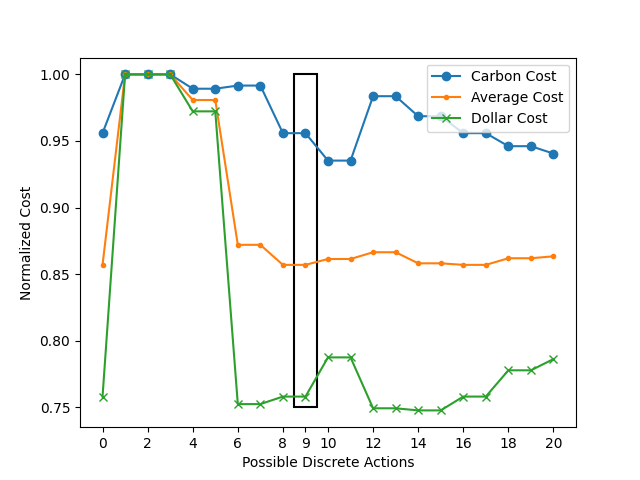
\includegraphics[width=\figurewidth]{figures/discretization.png}
  \caption{This graph shows the effect of the discretization resolution on the rule-based control algorithm. The coarsest resolution that does not significantly impact performance and includes the zero action is 9. In this graph, 0 possible actions means no discretization is applied.}
  \label{fig:discretization}
\end{figure}

In the pre-experiment on the effect of discretization, the rule-based agent performs comparably to the continuous case when discretization resolution is high, and worse on coarse resolutions. The coarsest resolution that performs similarly well as the continuous case is the subdivision into 8 or 9 possible actions.




\section{Hyperparameter Tuning}
All 200 runs of $\epsilon$-greedy DQN completed successfully.
10/100 runs of UA-DQN, all runs with a batch size of 1, failed.
18/200 runs of DQN-softmax failed, all of which share a batch size of 8.
However, 17 other runs with a batch size of 8 completed successfully.

Table \ref{tab:hyperparameters} shows the results of the tuning process for each algorithm.
For each algorithm, the learning rate had the most significant correlation with final performance, followed by the batch size and the target network update frequency.
The $\epsilon$ parameter of the optimizer Adam showed a large effect only for $\epsilon$-greedy DQN.

Figure \ref{fig:tuning_results} shows a histogram of the final performance of all successful tuning runs.
52\% of all UADQN runs perform better than the idle policy, 40.5\% of all DQN-softmax  runs perform better than the idle policy, and 37\% of e-greedy DQN runs perform better than the idle policy.

Both DQN algorithms show a peak at around -5000, which corresponds to strategies that are close to the idle policy.

\begin{table}[h]
  \centering
  \caption{This Table shows the correlation between tuned hyperparameters and algorithm performance for successful runs.}
  \label{tab:hyperparameters}
  \begin{tabular}{c||c|c|c}
    Algorithm & Hyperparameter & Value for Best Run & \makecell{Correlation with \\ final score} \\ \hline
    UA-DQN & Learning Rate                                & 3e-4 & \bf{-0.47}\\
           & Batch Size                                   & 128 &  0.28\\
           & Adam's $\epsilon$                            & 1e-07 & -0.03\\
           & \makecell{Target Network \\ Update Frequency}& 4 & -0.11\\ \hline
    DQN-Softmax & Learning Rate                                 & 3e-4 & \bf{-0.36} \\
                & Batch Size                                    & 128 & -0.18\\
                & Adam's $\epsilon$                             & 1e-05 & -0.02\\
                & \makecell{Target Network \\ Update Frequency} & 4 &  0.16\\ \hline
    $\epsilon$-greedy DQN & Learning Rate                       & 7e-05 & \bf{-0.33}\\
                & Batch Size                                    & 4 & -0.19\\
                & Adam's $\epsilon$                             & 1e-08 &  0.10\\
                & \makecell{Target Network \\ Update Frequency} & 16 &  0.14

  \end{tabular}
\end{table}



\begin{figure}
  \centering
  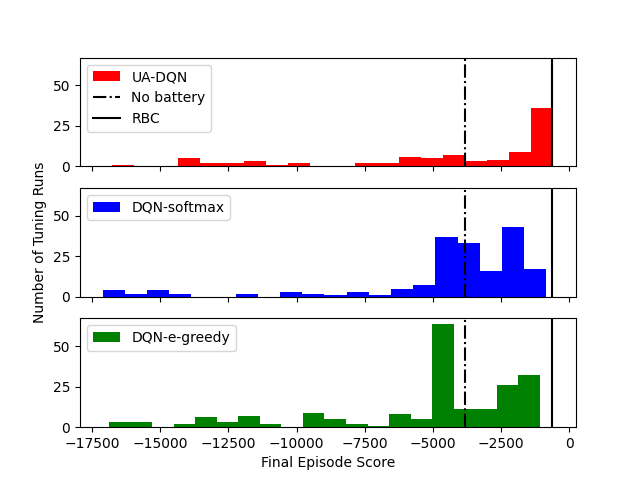
\includegraphics[width=\figurewidth]{figures/tuning_results.png}
  \caption{This histogram shows the final episode reward of all successful tuning runs. Every run represents one choice for the hyperparameters. The performance of the rule-based controller and the idle policy are shown for reference.}
  \label{fig:tuning_results}
\end{figure}

\section{Comparison of Tuned Algorithms}
\begin{figure}
  \centering
  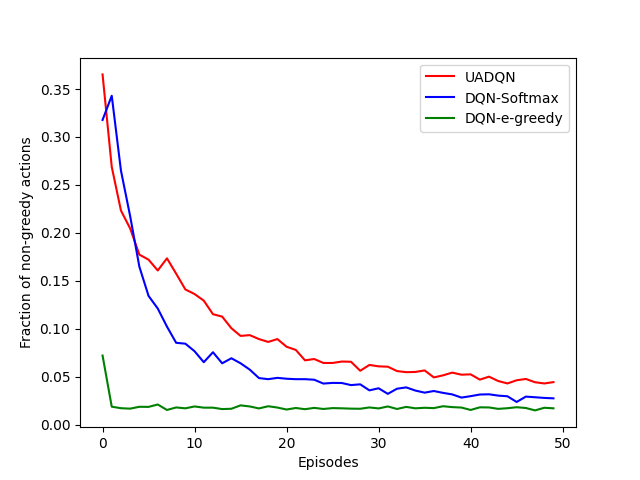
\includegraphics[width=\figurewidth]{figures/non-greedy-fraction.png}
  \caption{This graphic shows the exploration rate of tuned algorithms throughout the training process. It highlights the different action selection strategies employed by the different algorithms. UA-DQN keeps exploring for longer than the other strategies.}
  \label{fig:non_greedy_fraction}
\end{figure}
To illustrate the difference in exploration between the algorithms, figure \ref{fig:non_greedy_fraction} shows the fraction of selected non-greedy actions per episode.
All algorithms start out exploring more and then gradually decrease their exploration rate.
DQN-softmax and UA-DQN explore more than $\epsilon$-greedy DQN, which quickly reaches an exploration rate of $\epsilon = 0.02$.
UA-DQN keeps exploring more than the other algorithms.


Figure \ref{fig:tuning_validation} shows the episode rewards of the selected hyperparameters for each algorithm during training.
Tuned UA-DQN converges faster than the other algorithms, and it converges to a better mean performance, as shown in table \ref{tab:tuned_results}. The hand-engineered rule-based agent outperforms the tuned reinforcement learning algorithms on both metrics.

When repeated with 10 different seeds, a single run of DQN-softmax failed, compared to no failures from the other algorithms.


\begin{figure}
  \centering
  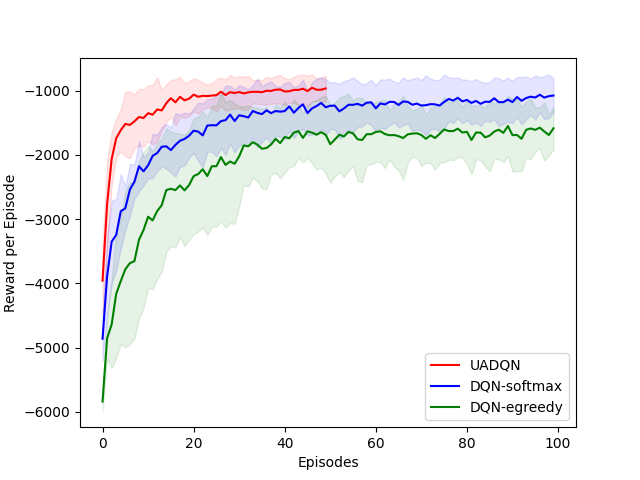
\includegraphics[width=\figurewidth]{figures/tuning_validation.png}
  \caption{This graphic shows the performance during training of the three tuned algorithms. The shaded area shows the standard deviation over 10 runs with different random seeds. Tuned UA-DQN converges after fewer episodes than either DQN variant. UA-DQN was only trained for 50 episodes due to the larger resource requirements of the algorithm.}
  \label{fig:tuning_validation}
\end{figure}

\begin{table}
  \centering
  \caption{This table shows the mean time per training episode for each of the tuned algorithms.}
  \label{tab:resources}
  \begin{tabular}[pos]{c|c}
    Agent & Mean Time per Training Episode \\ \hline           
    UA-DQN   & 95.3s \\
    DQN-Softmax  &27.2s \\
    $\epsilon$-greedy DQN &20.7s \\
  \end{tabular}
\end{table}

\begin{table}
  \centering
  \caption{This table shows the mean performance of tuned algorithms when evaluated using their respective action selection policy for one episode on Building 1.}
  \label{tab:tuned_results}
  \begin{tabular}{l|ccccc}
    Agent                 & Dollar Cost & Carbon Emission & Average \\ \hline
    Control (Idle)   & 1    & 1    & \textbf{1}    \\
    $\epsilon$-greedy DQN & 0.83 & 0.94 & $\mu = \mathbf{0.88}, SD = 0.017$ \\
    DQN-Softmax           & 0.83 & 0.93 & $\mu = \mathbf{0.88}, SD = 0.019$ \\
    UA-DQN                & 0.82 & 0.91 & $\mu = \mathbf{0.87}, SD = 0.010$ \\
    Discrete Rule-Based   & 0.80 & 0.88 & \textbf{0.84}
  \end{tabular}
\end{table}

\cleardoublepage

%%
%%%%%%%%%%%%%%%%%%%%%%%%%%%%%%%%%%%%%%%%%%%%%%%%%%%%%%%%%%%%%%%%%%%%
% Diskussion und Ausblick
%%%%%%%%%%%%%%%%%%%%%%%%%%%%%%%%%%%%%%%%%%%%%%%%%%%%%%%%%%%%%%%%%%%%

\chapter{Discussion}
  \label{Discussion}

Through the experiments described in the previous chapters, I evaluated the Uncertainty-Aware Deep Q Network algorithm on a custom building-scale energy-management environment based on the 2022 CityLearn challenge.
Compared to two versions of the simpler DQN algorithm, tuned UA-DQN requires fewer interactions with the environment to arrive at a good performance.
However, it does not reliably exceed the performance of a baseline rule-based control policy.
In this chapter, I discuss the collected evidence and limitations of the experiment and point out several possible ways of further improving the algorithm's performance.

\section{Preparation}
% Rule-Based Agent
% Summarize what I did
The baseline rule-based policy was manually derived from simple patterns observed in the data.
Its performance is compared to the performance of an idle policy, which does not make use the battery at all.
It enables substantial savings in electricity cost and carbon emissions.
% Interpret results
Compared to the idle policy, more of the generated solar electricity is used. \todo{maybe: report this stat: How much solar electricity is used in both cases, how much electricity is purchased in both cases?}
Therefore, overall, less electricity is purchased from the grid.
The policy also shifted the time of electricity purchase to an earlier time of day.
Especially during peak hours, when both price and carbon intensity are high, the policy achieves a substantial reduction in building electricity demand.
The policy does dynamically adapt to observed solar generation and electricity use, but it can not predict the amount of excess solar production to be stored, instead simply assuming it does not change from the hour before.
This is an obvious limitation of the policy.

Overall, the rule-based policy can serve as a useful baseline for evaluating the performance of more complex algorithms.
It is a simple algorithm that captures a lot of the storage potential of the system, but is not finely optimized on minute details.

% First Experiment: Discretization
% Summarize what I did
In order to determine the simplest discrete action space for the DQN variants that would allow them to perform well, I perform a pre-experiment on the rule-based policy.
The experiment tests the performance of the rule-based policy on different resolutions of discretized action space against its performance on the continuous action space.

% Discuss findings
Figure \ref{fig:discretization} shows a large dependency of the rule-based policy on resolution of the action space.
As expected, a higher discretization resolution approaches the continuous case and leads to better performance.
However, the policy's performance is particularly impacted by the fact that its minimum charging action of 0.24 in the hours before the high-price period starts is discretized into more or less useful values that for example don't fully charge the battery.


\section{RL Algorithms}
% Second Experiment: Tuning
% Summarize what I did
After establishing the baseline and environment details, I identify and tune important hyperparameters of UA-DQN and two versions of DQN for best performance.
I then rerun the tuned algorithms with multiple random seeds to get an estimate of their reliability.

% sensitivity to hyperparameters
The results of the tuning runs, presented in figure \ref{fig:tuning_results}, show that the performance of all algorithms depends on hyperparameter choice.
Comparing the algorithms, UA-DQN performs better for a wider range of hyperparameter choices.
For each algorithm, the most important hyperparameters are reported in \ref{tab:hyperparameters}. Across all algorithms, the learning rate is the most important hyperparameter as measured by correlation with the final score.
On average, a smaller learning rate leads to a better performance.
Adam's $\epsilon$ did not have a large effect on UA-DQN and DQN-Softmax, but tuning mattered on $\epsilon$-greedy DQN.

% general robustness
Some tuning runs failed. All UA-DQN runs with a batch size of 1 failed because the quantile Huber loss function needs a batch size of at least 2, but all other runs seemed to converge.
The DQN-Softmax algorithm failed to complete some runs with a batch size of 8. Even the tuned variant only completed 9/10 runs. This suggests some instability of the algorithm.

% action selection
Figure \ref{fig:non_greedy_fraction} shows the fraction of non-greedy actions taken by the tuned algorithms.
A non-greedy action is an action that was taken in order to explore the environment rather than exploit current knowledge.
UA-DQN explores more throughout the whole run than the other strategies.
$\epsilon$-greedy DQN explores much less than the other strategies.
A more sophisticated and tuned schedule for the exploration rate $\epsilon$ could improve the algorithm's performance at the added cost of requiring more tuning.

% general performance
Figure \ref{fig:tuning_validation} shows that UA-DQN improves its performance much faster than the other algorithms.
Especially in the first 5 episodes, when UA-DQN explores less than DQN-Softmax, UA-DQN performance improves much faster.
The reason for this could be either that tuned UA-DQN takes more useful exploratory actions, or that it integrates observed information more effectively, or a combination of both.

% Limitations of the experiment:
% Problems caused by tuning setup
The used tuning method favors risky hyperparameter choices.
Because every combination of hyperparameters is tried only once, accepting the single best tuning run probably means accepting an outlier performance for this combination of hyperparameters.
For example, the best performing runs of UA-DQN and DQN-Softmax share a low target network update frequency, which causes both faster learning and instability. Similarly, the best performing run of $\epsilon$-greedy DQN uses a small batch size of 4.
Therefore, the hyperparameters selected by the tuning process are biased towards being less reliable.
This effect might have helped UA-DQN, which was tuned for half as many runs as the other algorithms, so there was less opportunity for outliers to outperform more robust hyperparameters.
A different tuning procedure might have favored more reliable algorithms with a better mean performance.
One further possible source of bias is the networks' initialization, which was the same for all algorithms during tuning.

% Short summary
In summary, the experiment shows the potential of UA-DQN, which is able to take more useful exploratory actions.
The experiment suffers from multiple potential sources of bias, and a tuning procedure that favors unstable hyperparameters.
UA-DQN approaches the performance of the rule-based baseline and learns from fewer environment interactions than simpler DQN variants, but has much larger resource demands (see table \ref{tab:resources}).


\section{General Discussion}
% Limitations of the custom environment (external validity)
The custom environment based on the 2022 CityLearn challenge presents a planning and control task based on real-world data.
Some of the experiment's findings can be expected to generalize to real-world applications of the algorithms.
Particularly, the environment requires the agent to learn patterns in electricity price and carbon intensity, and domestic electricity usage and production.
The strategy task of when to use electricity storage is modelled well by CityLearn.
It depends on long-term, aggregate data and patterns on the scale of multiple hours.
In contrast, a part of the rule-based policy's idea is to store precisely the amount of excess electricity generated, which is nearly impossible to do in CityLearn, but easy to implement in a real-world building energy system.
This limits the effectiveness of a good long-term plan.

The environment used in the experiments only provided a subset of CityLearn's data as observed features.
For example, features included only one weather forecast variable, no information on day of the week or month, and no price forecasts.
Real-world weather forecasts are uncertain, which requires a different strategy for acting under uncertainty.
In a real-world application, a smart home system might also have access to occupant behavioral data, like knowing if someone is home or not, which can lead to significantly better plans.

While the building data stems from only one building in a particular climate zone, the algorithms' effectiveness depends mostly on the daily patterns of pricing.
More complex or dynamic pricing models might require more sophisticated planning algorithms.
In fact, coordination strategies such as dynamic pricing are another goal not addressed by this environment.
A real-world system could likely buy and sell electricity to and from the grid, providing flexibility not only to the building.

% CityLearn in general
The CityLearn framework is useful for developing experiments that test the application of RL planning algorithms to building energy control tasks.
It's an efficient environment that models important parts of a building and can incorporate real-world data.
However, in the current version, it does not serve as a realistic model for the full task.
Applying RL for building energy control is an area of ongoing research, and \cite{nweye2022RealworldChallengesMultiagent} name a number of challenges to be overcome when applying RL to grid-integrated buildings.

% General discussion: Can we answer the research questions?
The experiment described in this thesis shows that UA-DQN can explore a simple environment more efficiently than other RL algorithms.
This provides further evidence for the usefulness of uncertainty-aware RL methods when acting in high-stakes environments.
However, in this experiment, UA-DQN did not outperform the rule-based policy.
A real-life building energy demand response task might be more complex, which might favor a machine learning approach.

% Further research: See Conclusion


\todo[inline]{Maybe: Things I have not yet mentioned:
- UA-DQN needs a discrete action space.
- Talk about need for data: Interaction between replay buffer size and batch size.
- What would a good setting for the risk-aversion parameter even be?
}
\cleardoublepage

%%
%%%%%%%%%%%%%%%%%%%%%%%%%%%%%%%%%%%%%%%%%%%%%%%%%%%%%%%%%%%%%%%%%%%%
% Zusammenfassung
%%%%%%%%%%%%%%%%%%%%%%%%%%%%%%%%%%%%%%%%%%%%%%%%%%%%%%%%%%%%%%%%%%%%

\chapter{Conclusion and Outlook}
  \label{conclusion}
% Summary
UA-DQN is a Reinforcement Learning algorithm based on the DQN algorithm.
It learns the reward distribution and provides estimates for both epistemic and aleatoric uncertainty.
This allows it to explore more efficiently, and act according to a risk-aware strategy.
In this thesis, I apply the UA-DQN algorithm to a custom task for building energy management implemented in CityLearn.
I find that tuned UA-DQN outperforms two variants of DQN, reaching comparable performance with fewer environment interactions.
However, this added efficiency comes at a cost: UA-DQN has roughly three times as much computational cost as the simpler algorithms.
None of the tuned algorithms outperform an optimized rule-based control policy.

% Conclusions
Like other algorithms that explicitly represent uncertainty in addition to point estimates, UA-DQN is able to make use of this additional information.
Application of UA-DQN and similar algorithms should therefore be considered in problems where additional observations are expensive or bad decisions are costly.
Additionally, UA-DQN might perform particularly well on non-stationary problems, when local weather patterns or occupant behavior changes.
Future work can also generalize the method behind UA-DQN to a continuous action space.

CityLearn is a suitable framework to model a building energy management task for Reinforcement Learning, but it remains a challenge to transfer insights into real-world applications because of modeling and data decisions.
Future CityLearn challenges should play to its strengths and focus on longer-term planning rather than short-term control.
% Future work
In the context of automated Demand Response by building energy systems, there remain many exciting challenges for Uncertainty-Aware Reinforcement Learning.
One interesting line of work is multiagent learning and coordination mechanisms, as they will allow direct optimization for grid-scale goals.
Future work on uncertainty-aware Reinforcement Learning methods for building control should seek to incorporate uncertain data like weather forecasts or models of occupant behavior.
\cleardoublepage

%%%%%%%%%%%%%%%%%%%%%%%%%%%%%%%%%%%%%%%%%%%%%%%%%%%%%%%%%%%%%%%%%%%%%%%%%%%%%
%%% Appendix
%%%%%%%%%%%%%%%%%%%%%%%%%%%%%%%%%%%%%%%%%%%%%%%%%%%%%%%%%%%%%%%%%%%%%%%%%%%%%
\appendix

%\setcounter{secnumdepth}{-1}
%\section{Tables}\label{chap:App}
%\chapter{Further Tables and Figures}\label{chap:App}


%\cleardoublepage

%%%%%%%%%%%%%%%%%%%%%%%%%%%%%%%%%%%%%%%%%%%%%%%%%%%%%%%%%%%%%%%%%%%%%%%%%%%%%
%%% Bibliographie
%%%%%%%%%%%%%%%%%%%%%%%%%%%%%%%%%%%%%%%%%%%%%%%%%%%%%%%%%%%%%%%%%%%%%%%%%%%%%

\addcontentsline{toc}{chapter}{Bibliography}

\bibliography{mylit, papers}
%% Obige Anweisung legt fest, dass BibTeX-Datei `mylit.bib' verwendet
%% wird. Hier koennen mehrere Dateinamen mit Kommata getrennt aufgelistet
%% werden.

\cleardoublepage
%%%%%%%%%%%%%%%%%%%%%%%%%%%%%%%%%%%%%%%%%%%%%%%%%%%%%%%%%%%%%%%%%%%%%%%%%%%%%
%%% Erklaerung
%%%%%%%%%%%%%%%%%%%%%%%%%%%%%%%%%%%%%%%%%%%%%%%%%%%%%%%%%%%%%%%%%%%%%%%%%%%%%
\thispagestyle{empty}
\section*{Selbst\"andigkeitserkl\"arung}

Hiermit versichere ich, dass ich die vorliegende Masterarbeit 
selbst\"andig und nur mit den angegebenen Hilfsmitteln angefertigt habe und dass alle Stellen, die dem Wortlaut oder dem 
Sinne nach anderen Werken entnommen sind, durch Angaben von Quellen als 
Entlehnung kenntlich gemacht worden sind. 
Diese Masterarbeit wurde in gleicher oder \"ahnlicher Form in keinem anderen 
Studiengang als Pr\"ufungsleistung vorgelegt. 

\vskip 3cm
%Tübingen, 31.01.2023 \\
Ort, Datum	\hfill Unterschrift \hfill 
%%%%%%%%%%%%%%%%%%%%%%%%%%%%%%%%%%%%%%%%%%%%%%%%%%%%%%%%%%%%%%%%%%%%%%%%%%%%%
%%% Ende
%%%%%%%%%%%%%%%%%%%%%%%%%%%%%%%%%%%%%%%%%%%%%%%%%%%%%%%%%%%%%%%%%%%%%%%%%%%%%

\end{document}

